\chapter{果蝇活动台提取}
\label{chapter:container_split}

果蝇活动台提取步骤的输入包含多个果蝇活动台的视频,输出多个子视频,每个子视频均包含单独的果蝇活动台,为后续的果蝇行为分析做准备。果蝇行为视频的拍摄环境差异较大,用现有算法流程可能需要针对每个拍摄环境单独选择算法参数,为此本章在形状检测算法的基础上,提出了一种自适应的果蝇活动台提取算法。此外,现有的果蝇活动台提取算法往往存在较大的误差。为此,本文利用果蝇活动台之间固有的排列模式,提出了一种基于特定排列的果蝇活动台提取算法,提高果蝇活动台提取算法的准确性。

\section{活动台提取算法}\label{sec:container_split}

果蝇活动台一般是标准的圆形,分布在背景相对简单的拍摄场景中,可以根据活动台的形状进行提取。目前常见的果蝇活动台提取的标准算法流程一般包括:

\begin{enumerate}
\item 从视频中抽取$M$帧 $I_{k_1}, I_{k_2}, \ldots, I_{k_M}$,其中$M$的取值一般在$100\sim 1000$之间,$k_1, k_2, \ldots, k_M$表示视频帧的序号。为了尽可能的覆盖整个视频时长,对于$N$帧的视频,$k_1, k_2, \ldots, k_M$ 一般选取为$0\sim N$的等差数列,或者$0\sim N$中无放回的M次随机抽样;
\item \label{hough_step} 利用边缘检测算法得到$I_{k_1}, I_{k_2}, \ldots, I_{k_M}$的边缘,进而利用圆检测算法,找到视频帧$I_{k_1}, I_{k_2}, \ldots, I_{k_M}$中的圆。边缘检测算法可以选用Canny算子\cite{canny1986computational},圆检测算法可以选取Hough圆检测算法\cite{hough_circle_1990};
\item \label{container_center_step}对上一步骤中检测得到的圆的中心点坐标进行聚类,得到坐标中心的位置,即为活动台的位置。聚类中心的数目应等于果蝇活动台的数目。
\item \label{container_radius_step} 对\ref{hough_step}步骤中得到的圆的大小进行聚类,得到活动台的大小。因为果蝇活动台的构造一般包含2个圆,其中外侧圆限制了果蝇活动的范围,中心还有一个圆形凹槽用于投放果蝇食物,因而需要用聚类算法分别找到2个圆的大小。聚类中心的数目设置为每个果蝇活动台俯视图中圆形的数目;
\item \label{container_timeline_search}根据果蝇活动台的位置和中心,在原始视频中利用二分查找法,找到果蝇放入和移出视频的时间;
\item 利用\ref{container_center_step}, \ref{container_radius_step}, \ref{container_timeline_search} 的结果,逐帧对原视频进行切割,得到$M$个子视频。
\end{enumerate}

上述步骤涵盖了完整的果蝇活动台提取流程,其中,\ref{hough_step}步骤是关键步骤,Hough圆检测算法的结果决定了算法的准确性。但经验表明,果蝇活动台的边缘往往存在部分厚度或者阴影,利用Hough圆检测算法往往很难得到精确的解。为了使Hough圆检测算法找到数量足够、位置精确的圆,需要对算法参数加以优化。

Hough圆检测算法一般分为2步:首先对输入图像进行Canny边缘检测,其中参数$param_1$用于控制Canny算子的敏感度,$param_1$越小,对边缘越敏感;然后对图像进行Hough变换,得到参数空间中每个点对应图像空间中像素点的个数。为了减小参数空间的范围,可以设定半径的取值区间$[R_{min}, R_{max}]$;最后在特征空间中选取对应特征点数目超过$param_2$的极大值点作为检测结果,$param_2$参数值越小,检测到的圆的数目越多。随着$param_1$和$param_2$的减小,算法的对计算资源和内存资源的要求可能会急剧增加,此外,过低的$param_1$和$param_2$也有可能将更多的噪声信息误判为圆,从而影响到检测的准确性。

综上可知,可以通过调整活动台半径的范围$[R_{min}, R_{max}]$、$param_1$和$param_2$优化Hough圆检测的结果。活动台半径可以通过对视频分辨率和视频中摆放的活动台数目进行估算,也可以通过其他方式手动测量,在相同的拍摄环境下,果蝇活动台在视频中的尺寸是基本一致的,$[R_{min}, R_{max}]$也不需要重复配置。

$param_1$和$param_2$的设置可以通过自适应过程加以调整。首先,通过设置较大的$param_1$和$param_2$,对视频帧进行Hough圆检测,如果检测到的圆的数目和果蝇活动台的实际数目满足一定的条件,则认为找到了合适的$param_1$和$param_2$;否则,减小$param_1$和$param_2$,直到满足特定的条件为止。因为Hough算法的计算复杂度较高,在处理分辨率相对较高的输入视频时速度较慢,因而在对参数$param_1$和$param_2$进行自适应时,为了进一步降低计算复杂度,提高程序运行的效率,可以进一步降低对视频帧的采样数目,一般选取$30\sim 100$帧即可。

完整的果蝇活动台提取算法如算法~\ref{alg:container_split_adaptive}所示。
\begin{algorithm}
    \caption{自适应的活动台检测算法}
    \label{alg:container_split_adaptive}
\begin{algorithmic}[1]
\INPUT
    \Statex 果蝇行为视频;
    \Statex 活动台的数量$K_1$;
    \Statex 活动台圆的数量$K_2$;
    \Statex 活动台的最大可能半径$R_{max}$ 和 最小可能半径 $R_{min}$;
    \Statex Hough圆检测参数最大自适应次数$max\_iters$。
\OUTPUT
    \Statex 活动台的圆心$(x_1, y_1), \ldots, (x_{K_1},y_{K_1})$;
    \Statex 活动台的外径$R$;
    \Statex 活动台的移入时刻$t_{1, in}, \ldots, t_{K_1, in}$和移出时刻$t_{1, out}, \ldots, t_{K_1, out}$;
\State 从视频中抽取$M_1$帧视频$\{ I_{k_1}, I_{k_2}, \ldots, I_{k_{M_1}} \}$;
\State 初始化Hough圆检测的参数 $param_1^{\{0\}} = 200$, $param_2^{\{0\}} = 200$;
\For {$i = 0$ to $max\_iters$;}
    \State 对视频帧$\{ I_{k_1}, I_{k_2}, \ldots, I_{k_{M_1}} \}$,使用参数$param^{\{i\}}_1$和$param^{\{i\}}_2$进行Hough圆变换检测,得到$N_i$个圆;
    \If {$N_i < 3K_1$; }
        \State $param_1^{\{i+1\}} = 0.9\times param_1^{\{i\}}, param_2^{\{i+1\}} = 0.9\times param_2^{\{i\}}$
    \Else
        \State break
    \EndIf
\EndFor
\State 从视频中抽取$M_2$帧视频$\{ I_{l_1}, I_{l_2}, \ldots, I_{l_{M_2}} \}$
\State 使用参数$param_1 = param_1^{\{i\}}, param_2 = param_2^{\{i\}}$,利用Hough圆检测算法,对视频帧$\{ I_{l_1}, I_{l_2}, \ldots, I_{l_{M_2}} \}$进行圆检测,得到$N$个圆 $(\tilde{x}_1, \tilde{y}_1, r_1), \ldots, (\tilde{x}_N, \tilde{y}_N, r_N)$;
\State 使用GMM算法\cite{GMM_1999}将圆心$(\tilde{x}_1, \tilde{y}_1), \ldots, (\tilde{x}_N, \tilde{y}_N)$聚为$K_1$类,得到$(x_1, y_1), \ldots, (x_{K_1},y_{K_1})$;\label{alg:arena:clusterXY}
\State 使用GMM算法将半径$r_1, \ldots, r_N$聚为$K_2$类,得到$R_1, R_2, \ldots, R_{k_2}$,最终活动台的外径为$R = \max(R_1, R_2, \ldots, R_{k_2})$;\label{alg:arena:clusterR}
\State 检测$(x_i, y_i)$周围检测到的Hough圆的数目,利用二分查找法,分别查找$K_1$个聚类中心的移入视频的时刻$t_{i,in}$和移出视频的时刻$t_{i, out}$;
\State 输出$(x_1, y_1),\ldots,(x_K, y_K)$、$R$和$t_{1, in}, \ldots, t_{K_1, in}$以及移出时刻$t_{1, out}, \ldots, t_{K_1, out}$。
\end{algorithmic}
\end{algorithm}

通过自适应,可以提高果蝇活动台提取算法的鲁棒性,减少果蝇活动台提取步骤中的手工操作步骤。

\section{基于特定排列的果蝇活动台提取算法} \label{sec:container_split_fixed_array}

果蝇活动台提取算法的关键步骤在于Hough圆检测,而Hough圆检测算法的精确度往往比较差。为此可以依据果蝇活动台的排列情况,进一步校正活动台的位置。

在部分实验环境下,果蝇活动台被放置在特定的模具中,按照固定的方式排列,如图~\ref{fig:containers_fixed_by_array}所示。图~\ref{fig:containers_fixed_by_array}中,果蝇活动台呈矩形排列。利用果蝇活动台之间的位置信息,可以进一步提高果蝇活动台提取的准确性。一般来说,为了提高果蝇活动台的排列密度,果蝇活动台通常 按照矩形或正六边形进行排列,上述两种排列都很容易处理,下面仅以矩形排列为例,说明如何利用活动台的排列信息提高活动台提取的准确性。

\begin{figure}[htb]
\centering
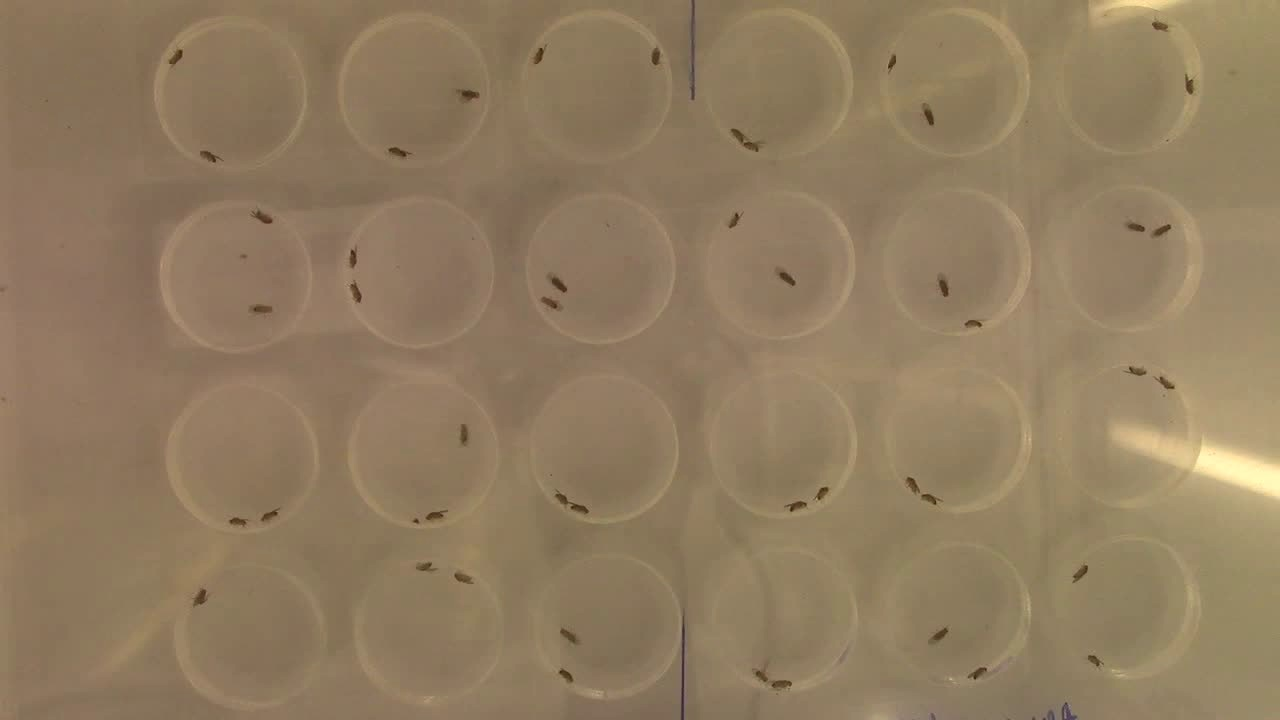
\includegraphics[width=0.8\textwidth]{containers_fixed_by_array}
\caption{按照矩形模式排列的果蝇活动台}
\label{fig:containers_fixed_by_array}
\end{figure}

在某些拍摄条件下,果蝇活动台的视频中存在较大的噪声,如图~\ref{fig:containers_fixed_by_array}所示,整个视频中的光照条件并不一致,图像的左侧亮度明显暗于右侧,整幅图中存在明显的阴影,右侧甚至存在清晰、明亮的光照情况,此外,果蝇活动台的侧壁也明显存在一定的模糊现象。上面的各种问题在多个拍摄场景中都有体现,尤其是果蝇活动台的边缘模糊,给Hough圆检测算法带来很大的影响,使得部分圆难以被准确检测到。此外,对检测到的圆心直接进行聚类时,受到噪声圆或聚类中心初始化的影响,聚类结果可能会有问题,使得部分活动台中心周围有不止一个聚类中心。利用果蝇活动台之间的排列关系可以一定程度上解决上述问题。下面介绍算法的具体过程。

首先,利用第\ref{sec:container_split}节中的自适应果蝇活动台提取算法,提取视频中果蝇活动台的大致位置,得到$K_1$个果蝇活动台中心$(x_1,y_1), \ldots, (x_{K_1},y_{K_1})$。

其次,根据果蝇活动台的排列方式,确定实际果蝇活动台在理想坐标系下的坐标$(\hat{x}_1, \hat{y}_1), (\hat{x}_2, \hat{y}_2), \ldots, (\hat{x}_{K_1}, \hat{y}_{K_1})$。当果蝇活动台按照图~\ref{fig:containers_fixed_by_array}所示进行排列时,在理想坐标系下,编号为$i$的果蝇活动台中心的位置为$(m_i, n_i)$,$m_i$和$n_i$分别表示该果蝇活动台所在的行数和列数。

再次,建立图像坐标系中坐标$(x_1,y_1),\ldots,(x_K,y_K)$和理想坐标系中坐标$(\hat{x}_1, \hat{y}_1), (\hat{x}_2, \hat{y}_2), \ldots, (\hat{x}_{K_1}, \hat{y}_{K_1})$之间的一一对应关系。首先,找到聚类中心的最小外包矩形;然后,将外包矩形旋转到某一边和坐标轴方向平行,并求出每个坐标方向上格点的距离;最后,根据每个格点的坐标,计算对应的行和列的位置,得到在理想坐标系下的坐标。在实际场景中,果蝇活动台的摆放方向和坐标轴基本平行时,可以省略上述求解外包矩形并旋转的步骤。

然后,建立从$(x_1, y_1),\ldots,(x_K, y_K)$到$(\hat{x}_1, \hat{y}_1), (\hat{x}_2, \hat{y}_2), \ldots, (\hat{x}_{K_1}, \hat{y}_{K_1})$的仿射变换。记仿射变换为$A$:
$$
A = \begin{bmatrix}
    a_{11} & a_{12} & a_{13} \\
    a_{21} & a_{22} & a_{23}
  \end{bmatrix}.
$$

根据映射关系,得到式(\ref{eq:img2ideal}):
\begin{equation} \label{eq:img2ideal}
\begin{bmatrix}
    a_{11} & a_{12} & a_{13} \\
    a_{21} & a_{22} & a_{23}
  \end{bmatrix}
\begin{bmatrix}
    x_{1} & x_2 & \ldots & x_K\\
    y_{1} & y_2 & \ldots & y_K\\
    1 & 1 & \ldots & 1
\end{bmatrix} =
\begin{bmatrix}
    \hat{x}_{1} & \hat{x}_{2} & \ldots & \hat{x}_K\\
    \hat{y}_{1} & \hat{y}_{2} & \ldots & \hat{y}_K
\end{bmatrix}.
\end{equation}

式(\ref{eq:img2ideal})共包含6个未知数,理论上需要3组坐标点即可求解。正常情况下,果蝇活动台的数目会超过3个,可以用最小二乘法求解式(\ref{eq:img2ideal})。为了便于表示,记
\begin{flalign}
P &= \begin{bmatrix}
    x_{1} & x_2 & \ldots & x_K\\
    y_{1} & y_2 & \ldots & y_K\\
    1 & 1 & \ldots & 1
\end{bmatrix}, \\
Q &= \begin{bmatrix}
    \hat{x}_{1} & \hat{x}_{2} & \ldots & \hat{x}_K\\
    \hat{y}_{1} & \hat{y}_{2} & \ldots & \hat{y}_K
\end{bmatrix},
\end{flalign}
得到$AP=Q$。根据最小二乘法,得到$A$的表达式:
\begin{equation}
A = QP^T(PP^T)^{-1}.
\end{equation}

最后,求解仿射变换$A$的逆变换$B$,即$B$变换将坐标从理想坐标系映射回图像坐标系,得到活动台的准确位置:
\begin{equation}
P' = BQ,
\end{equation}
其中
\begin{equation}
P' = \begin{bmatrix}
    \bar{x}_{1} & \bar{x}_{2} & \ldots & \bar{x}_{K_1} \\
    \bar{y}_{1} & \bar{y}_{2} & \ldots & \bar{y}_{K_1}
\end{bmatrix}.
\end{equation}

得到果蝇活动台准确的位置$(\bar{x}_1, \bar{y}_1), (\bar{x}_2, \bar{y}_2), \ldots, (\bar{x}_{K_1}, \bar{y}_{K_1})$后,对视频进行二分查找,得到果蝇活动台放入和移出的时刻,最后,根据果蝇活动台的位置、大小、放入时刻、移出时刻,对原始视频进行切割,得到单独的果蝇活动台视频。

果蝇视频的文件体积较大,一般需要对视频进行压缩。对于一个分辨率为1920$\times$1080、帧率为25帧的果蝇行为视频,完全无压缩的10分钟视频文件大小为84G,这就要求对果蝇行为视频采用适当的压缩。因为果蝇的身体尺寸较小,且果蝇的翅膀呈现半透明的特点,很容易因为视频压缩而损失视频信息。本文没有分析视频编码对果蝇行为分析结果带来的影响,所有的果蝇视频,包括原始输入视频和中间结果视频,均被保存为MPEG2-4格式。为了进一步提高果蝇行为识别的精度,可能需要进一步研究视频编码的影响。

\tikzstyle{block} = [rectangle, draw, text width=18em,  text centered, rounded corners, minimum height=3.5em]
\tikzstyle{arrow} = [thick, draw, -latex']

\begin{figure}[htb]
\centering
% 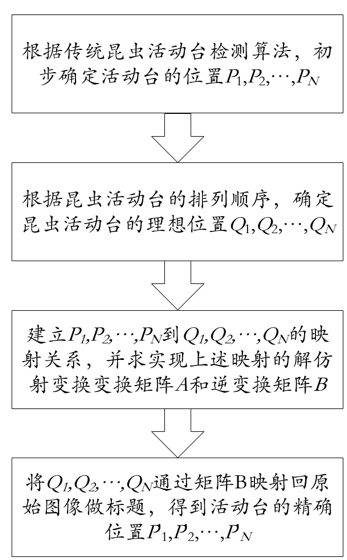
\includegraphics[scale=0.95]{fix_array_container_split}

\begin{tikzpicture}[node distance=2.5cm]

\node [block, minimum height=7em] (init) {\heiti 根据传统果蝇活动台检测算法,初步确定活动台的位置$P_1, P_2, \ldots, P_N$};
\node [block, below = 0.5cm of init, minimum height=7em] (idea_position) {\heiti 根据果蝇活动台的排列,确定果蝇活动台在理想坐标系下的位置$Q_1, Q_2, \ldots, Q_N$};
\node [block, below = 0.5cm of idea_position, minimum height=7em] (transform) {\heiti 建立$P_1, P_2, \ldots, P_N$到$Q_1, Q_2, \ldots, Q_N$的映射关系,并求解映射变换矩阵$A$和逆变换矩阵$B$};
\node [block, below = 0.5cm of transform, minimum height=7em] (inv_trans) {\heiti 将$Q_1, Q_2, \ldots, Q_N$通过变换$B$映射回原图像坐标系,得到活动台的精确位置$P'_1, P'_2, \ldots, P'_N$};

\path [arrow] (init) -- (idea_position);
\path [arrow] (idea_position) -- (transform);
\path [arrow] (transform) -- (inv_trans);

\end{tikzpicture}
\caption{基于特定排列的果蝇活动台提取算法流程}
\label{fig:fix_array_container_split_procedure}
\end{figure}

\section{果蝇活动台分割结果}

针对如图~\ref{fig:containers_fixed_by_array}所示的果蝇活动台,设置参数 $K_1 = 24, K_2 = 1, R_{max} = 80, R_{min} = 30, max\_iters = 15$,进行果蝇活动台提取。

首先对视频进行30帧采样,估算合适的$param_1$和$param_2$;然后,选取300帧视频进行Hough圆检测,如图~\ref{fig:simple_hough_circle}所示。从300帧视频中共计检测出了19658个圆,为了便于展示,在图~\ref{fig:simple_hough_circle}中仅包含随机抽取的394个圆。从图~\ref{fig:simple_hough_circle}中可以看出,Hough圆检测算法可以比较准确的找到活动台。但因为视频中存在不同的亮度等条件,造成圆检测结果的空间分布存在明显的不平衡,部分活动台周围有多个检测圆,而最下排第2和第4个活动台周围只有少量几个或者没有检测圆。此外,在视频的完全不相关位置也存在部分检测圆。这些都对果蝇活动台的提取带来干扰。

\begin{figure}[htb]
\centering
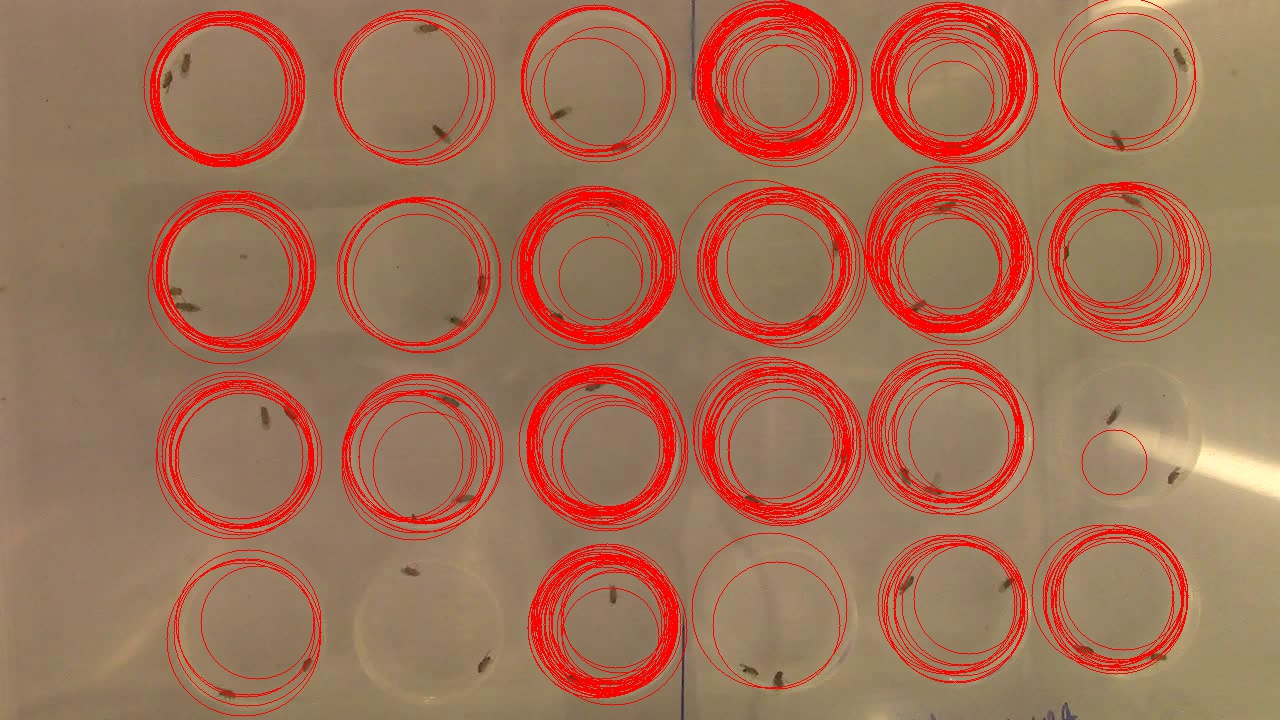
\includegraphics[width=0.8\textwidth]{simple_hough_circle}
\caption{Hough圆检测的结果}
\label{fig:simple_hough_circle}
\end{figure}

对Hough圆检测得到的圆进行聚类,得到如图~\ref{fig:containers_adaptive}所示的结果。图~\ref{fig:containers_adaptive}中显示的是\ref{sec:container_split}章中活动台提取算法的结果。参数$param_1$和$param_2$经过13次自适应后,最终取值为$param_1=param_2=56.5$,每个活动台周围平均检测到$3\sim 4$个Hough圆。从图~\ref{fig:containers_adaptive}可以看出,聚类后基本可以准确地找到活动台的位置,但是因为部分活动台周围仅能找到较少数目的Hough圆,且位置的准确性也存在较大的误差,因而检测结果与实际位置偏差较大。图~\ref{fig:containers_adaptive}中仅显示了检测结果不太准确的情况,在个别极端情况下,果蝇活动台提取算法还有可能出现漏检、重复检测的情况,即部分活动台被检出了2次,而有的活动台则一次都没有被检测到。通过选择足够多的视频帧、选取合适的聚类中心可以减少上述问题发生的概率,与此同时也会增加算法的计算量。

\begin{figure}[htb]
\centering
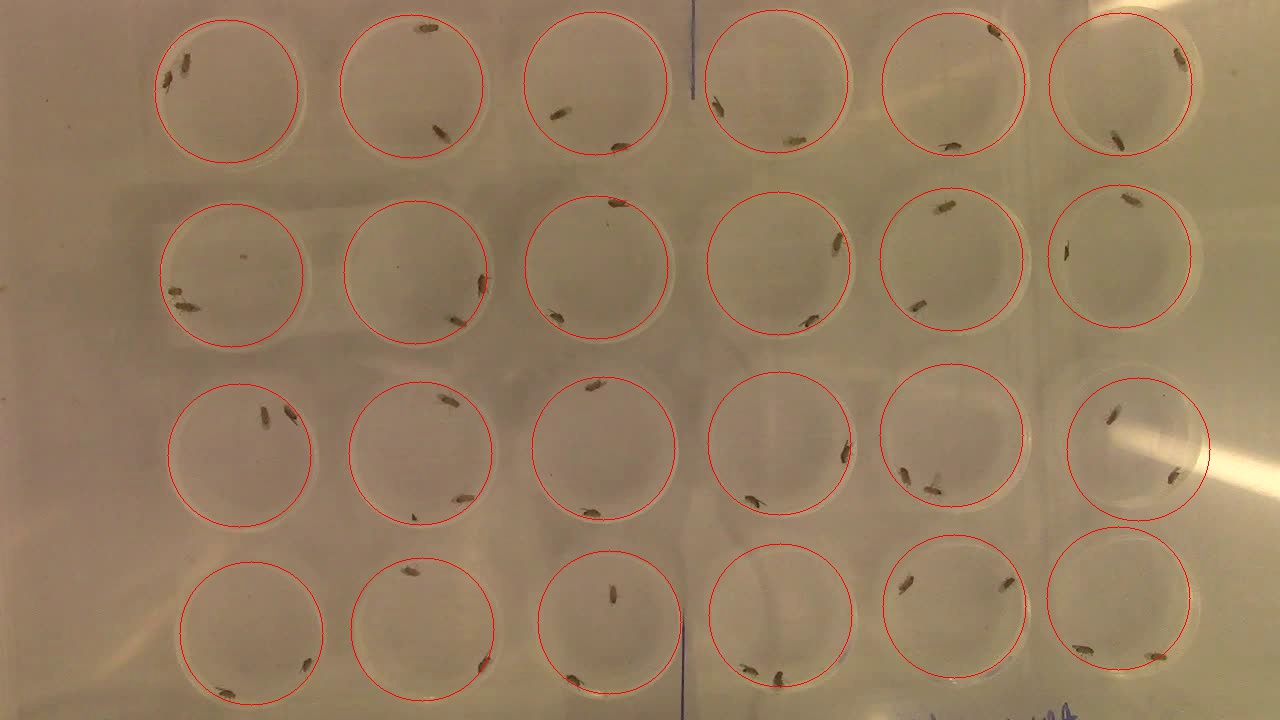
\includegraphics[width=0.8\textwidth]{containers_adaptive}
\caption{自适应的果蝇活动台检测结果}
\label{fig:containers_adaptive}
\end{figure}

最后,对图~\ref{fig:containers_adaptive}中的结果进一步采用基于固定排列的活动台提取算法,得到图~\ref{fig:containers_fixed_array}所示的结果。图~\ref{fig:containers_fixed_array}中果蝇活动台的位置和大小均比较准确。

\begin{figure}[htb]
\centering
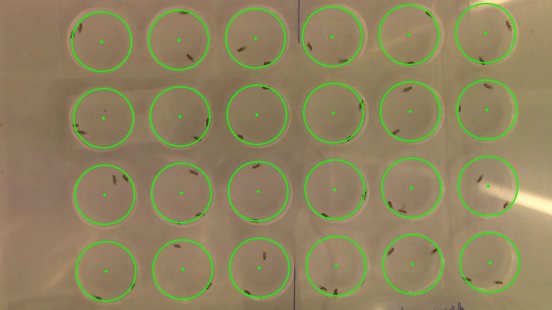
\includegraphics[width=0.8\textwidth]{containers_fixed_array}
\caption{基于特定排列的果蝇活动台检测结果}
\label{fig:containers_fixed_array}
\end{figure}

\section{小结}

本章主要介绍了果蝇活动台提取模块。首先介绍了基于形状检测算法的果蝇活动台提取算法,通过Hough圆检测参数的自适应,使得算法能较好的适应不同的视频。其次,基于特定排列模式的果蝇行为视频,通过对果蝇活动台位置进行建模,建立图像坐标系和理想坐标系之间的仿射变换,完成果蝇活动台位置的进一步优化。通过利用果蝇活动台的位置信息,提高了检测的准确性,提升了系统的可用性。最终完成果蝇活动台的切割,为接下来的果蝇轮廓提取做准备工作。
